%!TEX root =  ../main.tex

\subsection{Initial and Terminal}

\objective{Simplify angles and their coterminal synonyms, and apply them to the three basic trigonometric functions}


Angles are a measure of turning.  Since Babylonian times, it has been customary to divide
the circle into 360 parts, beginning directly off to the right, and proceeding counter-clockwise.
The beginning ray pointing right is known as the \textbf{initial side}, whereas the ray pointing
off where the angle has turned to is called the \textbf{terminal side}.

Because one direction of spin has been designated as positive, it is therefore true that
there exist negative angles.  These also begin at the initial side of $0^\circ$, but proceed
\emph{clockwise}.  Very quickly, there will be multiple names for the same angle.
Angle that end in the same place are called \textbf{coterminal}, after the Latin for the same.
Finding coterminal angles which are the same as a given angle is simply a matter of
adding or subtracting $360^\circ$ as many or as few times as desired.

Some processes in mathematic produce very large angle measures, which can become
cumbersome if dealt with by hand.  While it might be easy in some cases to simply
add or subtract $360^\circ$ until the angle is reasonable, this can become time prohibitive.
It is most efficient to find the remainder when an angle is divided by 360.

Degree/Minutes/Seconds will be dealt with in section §16.3, on sexigesimal numbers.

\subsection{Reference Angles}
Every angle can be thought of as a turn from the closest horizontal axis.  In the 
first quadrant, this is the angle itself, without modification.  In the fourth quadrant,
this is reversed, a certain distance down from $0^\circ$, or better, back from 
$360^\circ$.  For example, $330^\circ$ is an upside-down version of a $30^\circ$
angle, which is to say, the reference angle for $330^\circ$ is $30^\circ$.

In the second quadrant, things are not upside down, but mirrored.  What is the reference
angle for $150^\circ$?  Well the closest horizontal axis is not $0^\circ/360^\circ$, but
$180^\circ$.  The reference angle for $150^\circ$ is also $30^\circ$.  The third quadrant
is the hardest, being both flipped left-right, and up-down.  But $30^\circ$ past
$180^\circ$ is $210^\circ$.

\begin{figure}[h]
\begin{center}
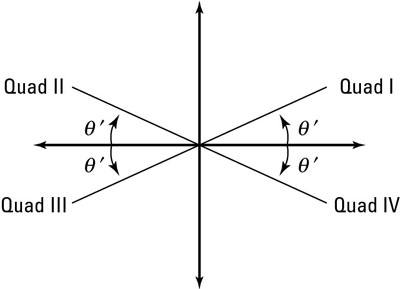
\includegraphics{reference}
\caption{Reference angles, sometimes call $\theta'$ (nothing to do with derivatives!)}
\end{center}
\end{figure}


\subsection{Trigonometric functions}
Also since ancient times, it has been exceedingly helpful to reference the ratios of
various components of an angle.  On a right triangle, these ratios are often memorized with
the helpful acronym S.O.H.C.A.H.T.O.A., short for sine = opposite/hypotenuse , cosine = 
adjacent/hypotenuse, tangent = opposite over adjacent.

\begin{figure}[h]
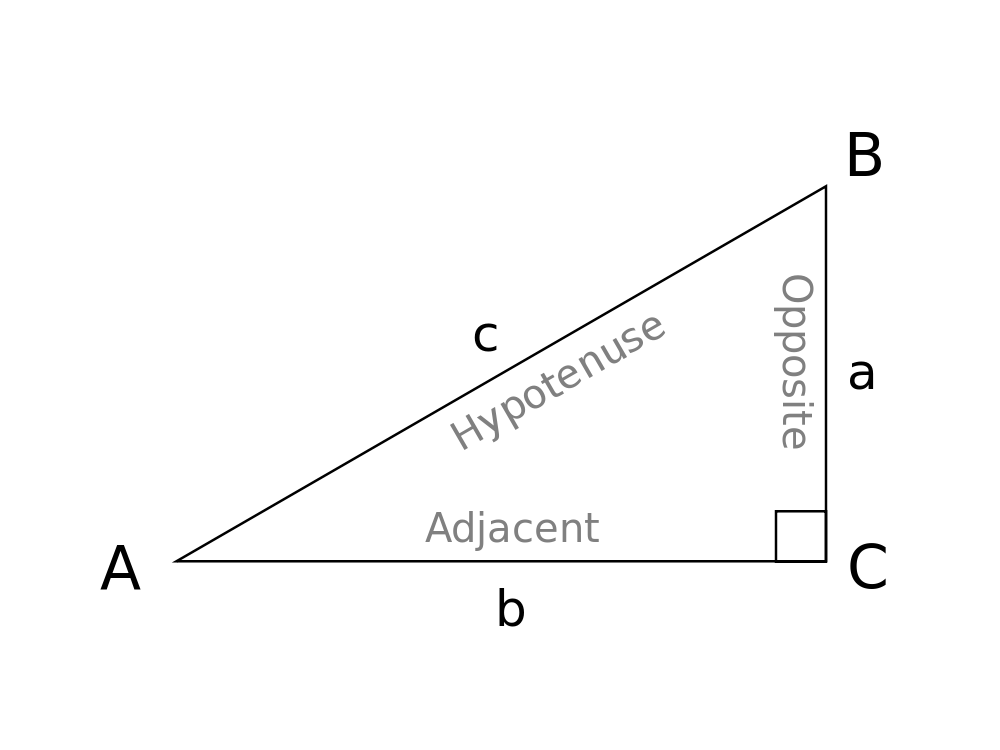
\includegraphics[scale=0.5]{TrigonometryTriangle.png}
\caption{The names of the sides of a right triangle}
\end{figure}

These definitions can be extended via reference angles to the other quadrants.  In 
such a context, the sine of an angle 
becomes the signed vertical displacement over the exact distance, cosine of an
angle becomes the signed horizontal displacement over the exact distance,
and tangent of the angle becomes its slope.

While no longer of much use or interest, there are names for the reciprocals of
the three main trigonometric functions.  The reciprocal of cosine is called
secant, the reciprocal of sine is called cosecant, and the reciprocal of tangent
is called cotangent.  Of these, only secant is commonly used (outside of math
classrooms!).

